\documentclass[border=10pt]{standalone}
\usepackage{pgfplots}
\usepgfplotslibrary{colormaps}
\pgfplotsset{trig format plots=rad}
\begin{document}
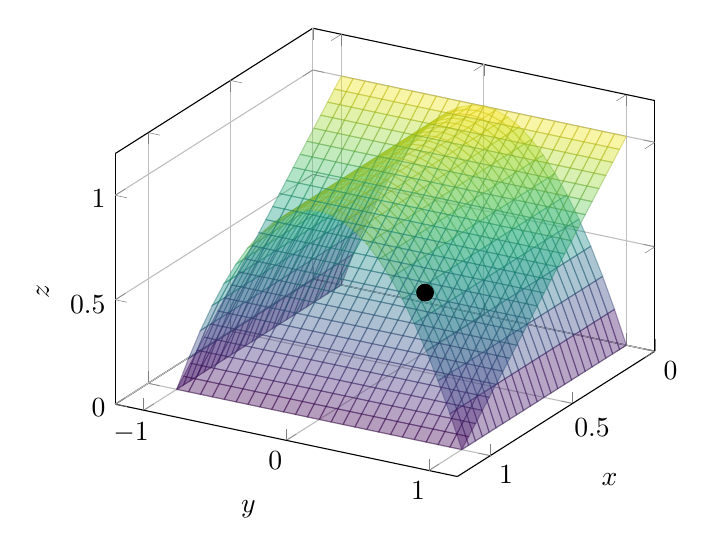
\begin{tikzpicture}
\begin{axis}[
    view={120}{30},
    xlabel=$x$, ylabel=$y$, zlabel=$z$,
    xmin=0, xmax=1.2,
    ymin=-1.2, ymax=1.2,
    zmin=0, zmax=1.2,
    grid=major,
]
% Plot the parabolic cylinder z = 1 - y^2
\addplot3[surf, opacity=0.4, domain=0:1, domain y=-1:1, samples=25, colormap/viridis] {1 - y^2};

% Plot the plane x + z = 1 => z = 1 - x
\addplot3[surf, opacity=0.4, domain=0:1, domain y=-1:1, samples=25, colormap/viridis] {1 - x};

% Center of Mass (approximate)
\addplot3[only marks, mark=*, mark size=3pt, color=black] coordinates {(0.357, 0, 0.286)};

\end{axis}
\end{tikzpicture}
\end{document}
